\section{Generalisation: two nulls and one failure}
\label{sec:generalisation}

Once a single feature reached \nFloorM{}, the headline AUC could no longer show that a model had
learned anything a one-line rule could not. Two experiments were meant to carry that weight
instead: leave-one-country-out, and a fraud sub-variant that appears only in the test period.
Both are null. This section reports them as null results rather than dropping them, explains why
this benchmark could not make them informative, and reports the one experiment that did find a
failure.

\subsection{Leave-one-country-out}

Each country is removed from training entirely and then scored, and each result is compared with
the same country scored by the model that saw it (Table~\ref{tab:loco}). Removing a country costs
at most \nLocoMaxLoss{} AUC; on the earlier draw \texttt{6abde44e} it cost at most
\nEarlyLocoMaxLoss{}.

\begin{table}[htbp]
\centering
\caption{AUC per country, in-sample and with the country unseen in training (diagnostic model,
draw \texttt{d8083dbc}, \nBatTestRows{} test rows, evidence commit \texttt{d40fca2}, source
\texttt{docs/benchmarks/m4\_battery\_d8083dbc\_e1.txt}). CD rests
on fewer than 30 fraud rows and gives direction only.}
\label{tab:loco}
\begin{tabular}{lrrr}
\toprule
Country & In-sample & Unseen in training & Fraud rows \\
\midrule
KE & \nLocoKEin & \nLocoKEout & \nLocoKEf \\
RW & \nLocoRWin & \nLocoRWout & \nLocoRWf \\
TZ & \nLocoTZin & \nLocoTZout & \nLocoTZf \\
UG & \nLocoUGin & \nLocoUGout & \nLocoUGf \\
CD & \nLocoCDin & \nLocoCDout & \nLocoCDf \\
\bottomrule
\end{tabular}
\end{table}

The null has a mechanism, and it is tested rather than argued: \textbf{no fraud parameter is keyed
by country} (a test fails if one is). Country enters only as a lookup for which mule, merchant,
agent, currency or time zone an incident uses, so withholding a country withholds no fraud
mechanism. Country-level generalisation cannot be evaluated on this benchmark and belongs to a
real-data validation plan. We did not change the generator to make countries differ: no source
read gives fraud prevalence by type and country for these markets, so the only way to choose such
a parameter would be to pick whatever makes the experiment show a gap, which defines the ground
truth from the test's desired answer (ADR 0028).

\subsection{A novel variant held out in time}

\texttt{novel\_esim\_delayed\_drain} occurs only in the test period. All variants are scored
against the same legitimate rows at one threshold, the \nFPRBudget{} false-positive budget over all
legitimate rows. The unseen variant is caught at \nNovelRecall{} \nNovelCI{} (\nNovelCaught{} of
\nNovelRows{}), against \nBaseVarRecall{} \nBaseVarCI{} for the base scenarios the model trained
on: at least as often as the familiar shape. On the earlier draw the figures were
\nEarlyNovelRecall{} against \nEarlyBaseRecall{}. The variant's novelty is in its lead time (a
drain delayed by days rather than minutes after the enabling SIM event), not in its transaction
pattern, which is still a burst, so a model that detects bursts catches it without having seen it.
This is not an out-of-distribution test.

\subsection{One cause}

Both nulls, and the redundancy of Section~\ref{sec:redundancy}, have one explanation: \textbf{the
benchmark encodes fraud as bursts}, and every country, every variant and every feature group is a
view of that single structure. What the benchmark supports is detection \emph{given}
burst-structured fraud, and the cost of computing and explaining that detection. It supports no
claim about generalisation, geographic or temporal.

\subsection{A pre-registered non-burst variant: the one failure found}

A generalisation test needs a mechanism that actually differs, and the ``sent by mistake'' reversal
scam is one. Its ingredients are documented among Kenyan M-PESA users. In a survey of them,
forged M-PESA confirmation messages were the most common scam reported \cite[Section~5.1.1]{dogan2025grift};
the same study notes that M-PESA's business services block reversals to foil opportunistic and
malicious reversal requests \cite[Section~2]{dogan2025grift}, and one respondent reported asking
the sender to reverse an apparently mistaken transfer \cite[Section~5.3.3]{dogan2025grift}. The scam itself
is described in the Kenyan press: the victim receives a fake M-PESA message that shows ``LOCKED''
where the balance should be, the scammer claims to have sent the money by mistake, often with an
emotional story, and the victim sends it back, only to find that no money was ever deposited;
Safaricom's advice, quoted there, is not to refund the money \cite{star2025mpesa}. The victim's
loss is therefore a single transfer that the victim initiates, to the number of the claimed sender.
Neither source says whether the victim has paid that number before; since it is the scammer's own
number, we read the documented form as a transfer to a new counterparty.

The benchmark's variant keeps the single, victim-initiated transfer and departs from that form in
one deliberate respect: its recipient is a counterparty the victim already knows. That is a
modelling choice, not a property the sources describe (ADR 0028). It removes both axes this
benchmark's detection relies on at once, burst structure and counterparty novelty, which makes the
variant the harder case of the two: the documented form, with its new recipient, keeps counterparty
novelty. The generator stages each such row as a \texttt{mule\_account} row with its own sub-variant
label (Table~\ref{tab:scenarios}).

The variant's definition, its justification and the predicted result were committed before the
dataset was regenerated and before any measurement existed (ADR 0028). The prediction: recall at
the same threshold \textbf{between \nRevPredLow{} and \nRevPredHigh{}}, lower than the base
scenarios but not zero, with recall below about \nRevPredFloor{} stated as the outcome that would
say burst structure and counterparty novelty carry nearly all of the benchmark's detection power.

\textbf{Result.} \texttt{reversal\_scam\_social\_engineering} is caught at \nRevRecall{}
(\nRevCaught{} of \nRevFraud{}, Wilson \nRevCI{}), against \nBaseVarRecall{} \nBaseVarCI{} for the
base scenarios on \nBaseVarFraud{} rows; its AUC is \nRevAUC{}. The intervals do not overlap.
The denominator is \nRevFraud{} rather than the \nRevRows{} rows the generator wrote because the
evaluation reads the observed label, as a deployed model would: all \nRevTrueFraud{} rows are in
the test period and are fraud by their true label, and \nRevScoredUnlabelled{} of them carry the
benchmark's missed-fraud label noise (Section~\ref{sec:dataset}), so they are scored as legitimate
rows (\texttt{evidence/\allowbreak reversal\_\allowbreak labels\_\allowbreak d8083dbc.txt},
Appendix~\ref{app:evidence}). The
point estimate is below the pre-registered range; the interval now reaches past the range's lower
edge, so ``below the predicted range'' holds for the point estimate and not for the whole interval.

\begin{figure}[htbp]
\centering
% Generated by figures/make_figures.py from numbers.tex; do not edit.
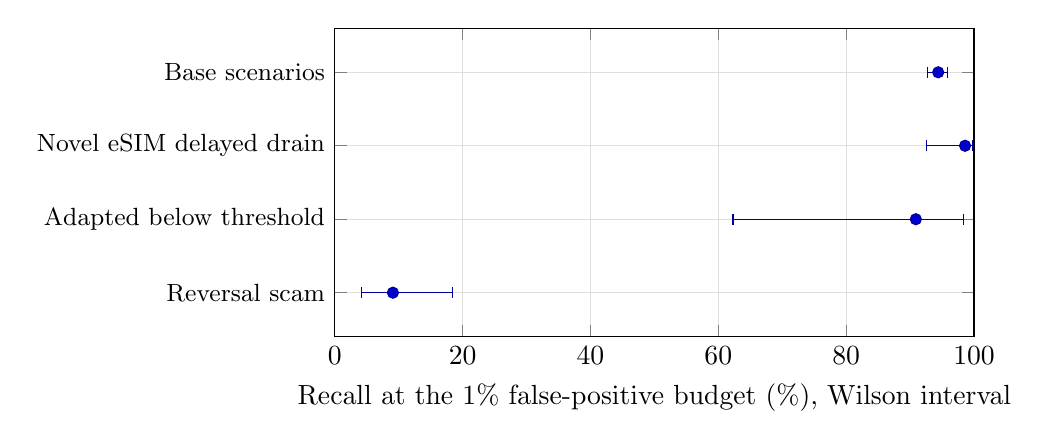
\begin{tikzpicture}
  \begin{axis}[
      width=0.8\linewidth, height=5.5cm,
      xmin=0, xmax=100, xlabel={Recall at the 1\% false-positive budget (\%), Wilson interval},
      symbolic y coords={{Base scenarios},{Novel eSIM delayed drain},{Adapted below threshold},{Reversal scam}},
      ytick=data, y dir=reverse, yticklabel style={font=\small}, enlarge y limits=0.2,
      grid=major, grid style={gray!25},
    ]
    \addplot+[only marks, mark=*, blue!60!black,
      error bars/.cd, x dir=both, x explicit] coordinates {
      (94.4,{Base scenarios}) -= (1.7,0) += (1.4,0)
      (98.6,{Novel eSIM delayed drain}) -= (6.0,0) += (1.2,0)
      (90.9,{Adapted below threshold}) -= (28.6,0) += (7.5,0)
      (9.1,{Reversal scam}) -= (4.9,0) += (9.3,0)
    };
  \end{axis}
\end{tikzpicture}

\caption{Recall of each fraud variant at the same threshold, with Wilson intervals (diagnostic
model, draw \texttt{d8083dbc}, \texttt{docs/benchmarks/m4\_battery\_d8083dbc\_e1.txt}). Generated by
\texttt{figures/make\_figures.py} from \texttt{numbers.tex}.}
\label{fig:variants}
\end{figure}

\textbf{A correction, reported rather than hidden.} The first measurement gave \nRevRecallFirst{}
\nRevCIFirst{} (\nRevCaughtFirst{} of \nRevFraud{}; AUC \nRevAUCFirst{}) against
\nBaseVarRecallFirst{} \nBaseVarCIFirst{}. It used a random-fold target encoding, which the project's rule that
every fold, split, sample and encoding groups by account (E1) forbids; re-running on the same data with the permitted encoding produced the
figures above. The conclusion did not change; the interval did.

\textbf{What this does and does not show.} It confirms, on a held-out shape rather than by inference
from ablation margins, that when burst structure and counterparty novelty are both absent the
remaining signals (amount, channel, time) do not recover this benchmark's detection power. Because
the variant removes the two axes together, the result cannot say how much each contributes on its
own; a variant with a new recipient, as in the documented form, would separate them and has not
been measured. It does not show that non-burst fraud is undetectable: other typologies are
untested, and a real system has signals this benchmark does not simulate. A second
held-out variant, \texttt{adapted\_below\_threshold}, rests on \nAdaptFraud{} fraud rows (recall
\nAdaptRecall{} \nAdaptCI{}); its interval overlaps the base scenarios' and establishes nothing on
its own.
